\documentclass[tikz,border=6pt]{standalone}
\usepackage{amsmath,amssymb}
\usetikzlibrary{arrows.meta,calc,decorations.markings}

\begin{document}
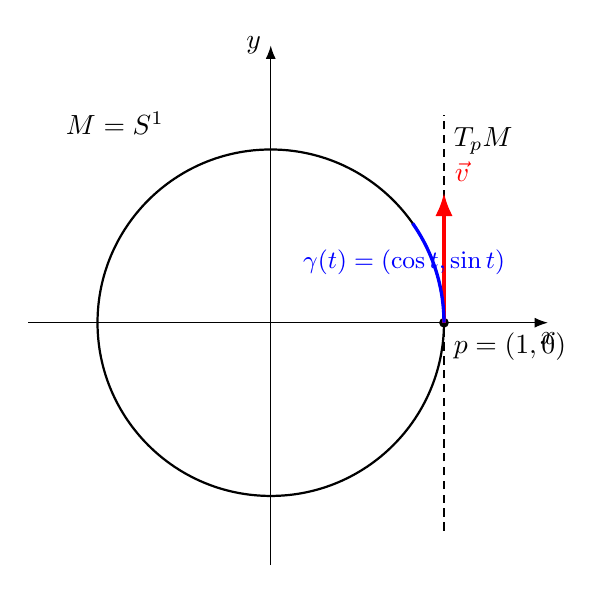
\begin{tikzpicture}[scale=2.2,>=Latex]
	
	% Axes
	\draw[->] (-1.4,0) -- (1.6,0) node[below] {$x$};
	\draw[->] (0,-1.4) -- (0,1.6) node[left] {$y$};
	
	% Unit circle
	\draw[thick] (0,0) circle (1);
	\node at (-0.9,1.15) {$M=S^1$};
	
	% p and tangent line
	\coordinate (p) at (1,0);
	\fill (p) circle (0.8pt);
	\node[below right] at (p) {$p=(1,0)$};
	
	\draw[densely dashed] (1,-1.2) -- (1,1.2);
	\node[right] at (1,1.05) {$T_pM$};
	
	% v
	\draw[very thick,red,->] (p) -- ++(0,0.75) node[above right] {$\vec v$};
	
	% gamma arc
	\draw[very thick,blue] (1,0) arc[start angle=0,end angle=35,radius=1];
	\node[blue] at (0.77,0.35) {\small $\gamma(t)=(\cos t,\sin t)$};
	
\end{tikzpicture}
\end{document}